\section{Iterative algorithm for center of mass displacement compensation}\label{sec:Algorithm}
In reality, the distribution of the mass within the body is not known, and therefore, an analytic solution provided with (\ref{eq:CMsolution2}) is impossible to obtain, thus an iterative method, based on repetitive hopping response is proposed. Prior to the jump, the quadruped rests on the flat surface. In order to initiate the jump, the legs apply the infinitesimaly short thrust and consequently, reaction forces and torques acting on the body can be approximated with the Dirac function $\delta (t)$. During the jump, the body behaves according to the Euler body dynamics function (\ref{eq:EulerBody}). Taking into account the infitessimally short time the body has to accelerate (i.e. the rotation speeds are small, and their product is even smaller) the cross coupling term $\vec{\boldsymbol{\omega}}\times \textbf{J}_B\vec{\boldsymbol{\omega}}$ can be neglected and, consequently, the rotation speed vector can be approximated with (\ref{eq:RotSpeedAprox}).
\begin{figure}
	\centering
	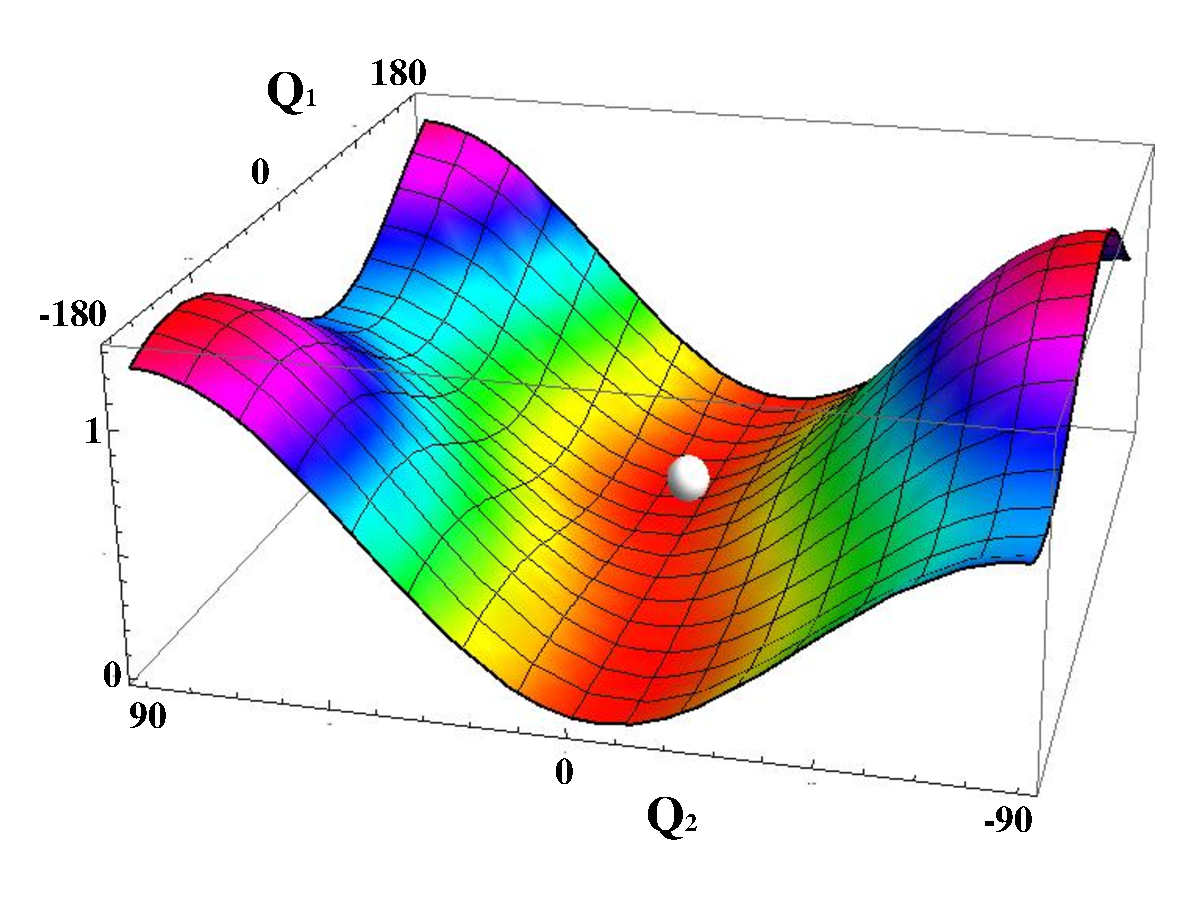
\includegraphics[width=85mm]{./pictures/RobinRepicCM.pdf}
	\caption{Center of mass displacement}
	\label{fig:CM3Dfunction}
\end{figure}

\begin{equation}\label{eq:EulerBody}
\vec{\boldsymbol{\tau}_{tot}}=\textbf{J}_B\vec{\dot{\boldsymbol{\omega}}}+\vec{\boldsymbol{\omega}}\times \textbf{J}_B\vec{\boldsymbol{\omega}}
\end{equation}

\begin{equation}\label{eq:RotSpeedAprox}
\vec{\boldsymbol{\omega}}\approx \frac{1}{s}{\textbf{J}_B}^{-1}\begin{bmatrix}
\Delta \textsc{y}_{CM} & -\Delta \textsc{x}_{CM} & 0
\end{bmatrix}^T\bar{T}\delta(s)
\end{equation}

Calculating the absolute value of vector (\ref{eq:RotSpeedAprox}) it is easy to show that the size of the rotation speed vector is proportional to the displacement of center of mass \eqref{eq:WpropCM}. In other words, centering the robot and minimizing the displacement of the center of mass eliminates the generation of unwanted rotations. 

\begin{equation}\label{eq:WpropCM}
\left \| \vec{\boldsymbol{\omega}} \right \|\sim \sqrt{{\Delta \textsc{x}_{CM}}^2+{\Delta \textsc{y}_{CM}}^2}
\end{equation}


In order to iteratively calculate the angles $q1$ and $q2$, angular velocity vector is recorded during the hopping acceleration phase. In order to start the jump procedure, the initial actuated spring value $L_{i0}$ is changed for a small value $\Delta L$:

\begin{equation}
\tiny
L_{i1}=L_{i0}+\Delta L
\normalsize
\end{equation}  

This phase is completed ($t_{JC}$) when one of the legs/springs reaches the desired length $L_{i1}$. The leg which carries a minimum weight (i.e. attached to a cuboid of minimal mass) will achieve the fastest accelerations and the algorithm’s task is to navigate the tail towards this leg. At the end of the acceleration phase the body rotates with an angular velocity $\vec{\boldsymbol{\omega}}(t_{JC})$. By using the cross product of the projection vector $\vec{\boldsymbol{\omega}_{xy}}$ in $XY$ plane and the body $\vec{\boldsymbol{Zb}}$, the tail direction vector $\vec{\boldsymbol{\omega}_{TD}}$ is calculated (see Fig.\ref{fig:imassCom}). The tail motion control algorithm navigates the tail in $\vec{\boldsymbol{\omega}_{TD}}$ direction by using the simple P($K_o$) controller. The algorithm finishes when $\left \| \vec{\boldsymbol{\omega}}(t_{JC}) \right \|\ $ is smaller than the  predefined limit value $\omega_{max}$.  For example, the mass distribution in Fig.\ref{fig:imassCom} is equally distributed except for $m_2$  which is lighter than the others. As expected, the iterative algorithm will navigate the tail towards that mass.



\begin{algorithm}
\caption{Minimize $\left \| \vec{\boldsymbol{\omega}} \right \|\sim \sqrt{{\Delta \textsc{x}_{CM}}^2+{\Delta \textsc{y}_{CM}}^2}$}
\begin{algorithmic} 
\STATE $y \leftarrow 1$
\REPEAT
\STATE $q_1 \leftarrow$ initial value
\STATE $q_2 \leftarrow$ initial value
\STATE JUMP

\REPEAT
\STATE recording $\vec{\boldsymbol{\omega}}(t)$
\UNTIL JUMP COMPLETE
\STATE $\vec{\boldsymbol{\omega}_{TD}} = \vec{\omega_{xy}}(t_{JC}) \times \vec{\boldsymbol{Zb}}$
\STATE Move tail in $\vec{\boldsymbol{\omega}_{TD}}$ direction - gain $K_o$
\UNTIL{$\left \| \vec{\boldsymbol{\omega}}(t_{JC}) \right \|\ < \omega_{max}$}
\end{algorithmic}
\end{algorithm}


\begin{figure}
	\centering
	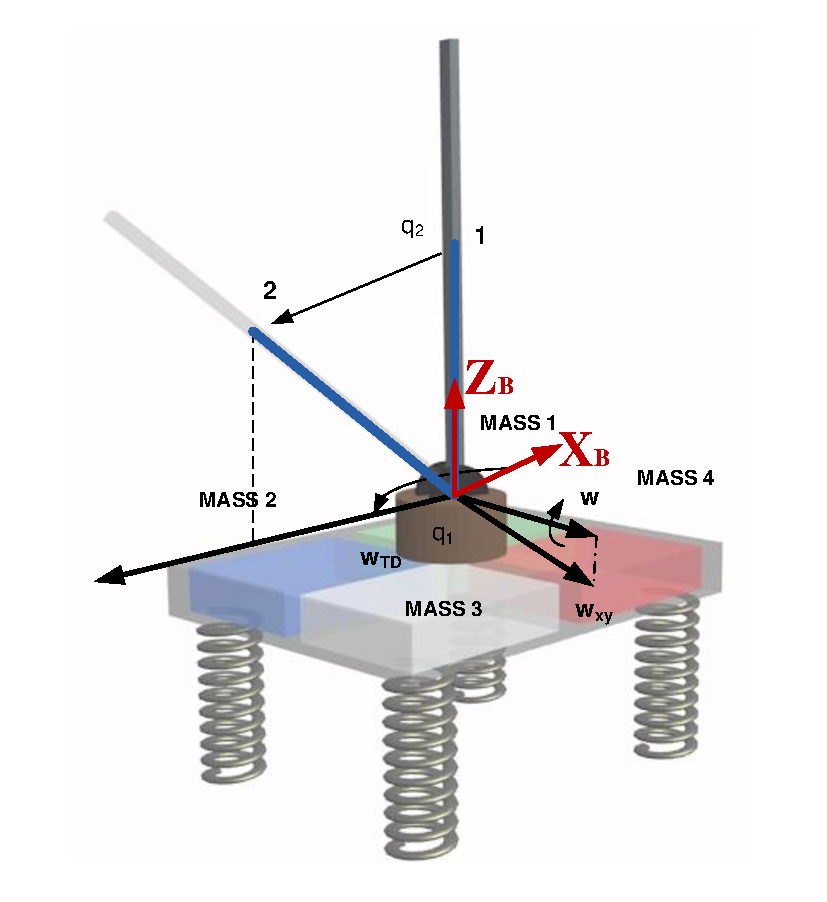
\includegraphics[width=85mm]{./pictures/IterativeAlgorithm.pdf}
	\caption{Iterative mass displacement compensation}
	\label{fig:imassCom}
\end{figure}
